\chapter{基于复合抽样的分布式轨迹聚类算法}

%已研究的缺点:
%1.需要数据聚集,不符合场景和隐私
%2.统计信息+代表向量
%3.概率模型
%4.网络带宽

\section{引言}
目前针对分布式聚类算法的研究已经取得了一些成果,一部分研究方法是以数据聚合为前提的,比如文献\cite{FanA}和文献\cite{Wang2018A}提出的方法,这类方法首先需要将分布式中的数据集合在一起,然后以特定的方式将数据集划分给各个属地节点以提高聚类准确度和计算高效性,这类方法在聚类准确度上和数据集中式聚类相当,但是由于需要原始数据在网络中传输,这使得该算法在很多需要考虑数据隐私性的场景下变得不适用;鉴于数据隐私层面的考虑,一部分研究基于安全多方计算提出了自定义用于分布式计算加密协议,这类方法虽然在数据隐私层面和聚类准确度上表现良好,但却消耗了大量的带宽资源,特别是对于在数据量爆炸式增长的今天。

另一部分研究主流思路是基于局部聚类和全局聚类相结合的方式\citing{Januzaj2004Scalable}\citing{郑苗苗2007DK}\citing{merugu2003privacy},其主要思想为:在分布式框架中有两种角色,若干个属地节点和一个中心节点,属地节点基于本地的数据先进行局部聚类,然后依据局部聚类结果和一些额外的统计信息组成特定的数据结构,各个属地节点将由局部聚类结果和统计信息组成的数据结构通过网络传输给中心节点,中心节点利用局部聚类结果进行全局聚类,然后将全局聚类结果传输给各个属地节点。这类方法由于其在计算准确度、带宽和隐私性层面三方面的平衡,受到了很多学者的青睐,但这类算法的计算准确度不太稳定,造成这种不稳定的原因是这类方法在网络中传输的数据结构与数据的真实分布不是一一映射的关系,一个属地节点利用局部聚类结果和统计信息组成的数据结构可能对应多种数据分布,而这种映射到数据分布的多样性将给后续的全局聚类造成影响,数据结构到数据分布的多样性如图\ref{diversity}所示。
\begin{figure}[h]
	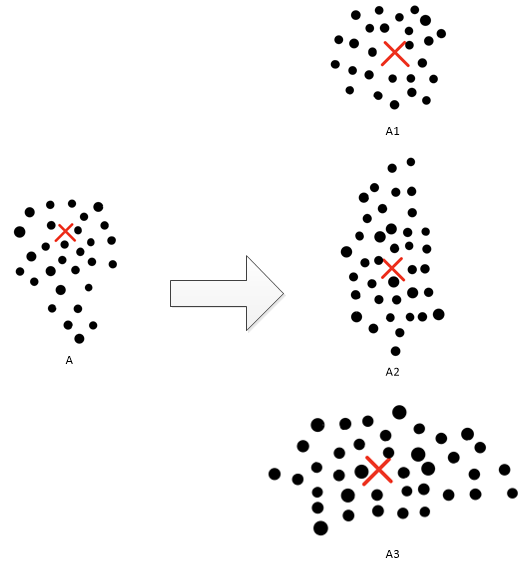
\includegraphics[width=0.6\textwidth]{diversity.png}
	\caption{数据结构到数据分布映射的多样性}
	\label{diversity}
\end{figure}

图中红色叉表示局部聚类得到的簇心,A对应的是真实数据分布,而A1、A2和A3对应的数据分布与A对应的数据分布有着同样的数据结构(簇心和统计信息),即一个数据结构(簇心和统计信息)对应着多种数据分布,而不同的数据分布可能使得全局聚类的结果迥然不同。针对这种情况,本文提出一种基于复合抽样的分布式轨迹聚类算法(CSD-Clustering),该算法为每一条抽样轨迹建模,在网络中传输的是每一条抽样轨迹的模型参数,算法聚类准确度高且聚类结果稳定性强,且通过复合抽样操作有效控制了网络流量的消耗。

\section{基于复合抽样的分布式轨迹聚类算法}

\subsection{问题建模}
首先简述基本的符号定义和距离定义,然后给出隐私相关描述和设计目标。

假设多属地分布式系统中,有k个跨地理分布的属地节点,包含一个中心节点。每个属地节点拥有m条时空轨迹数据。对于每条时空轨迹,其中有n个数据点,表示数据对象以时间顺序经过了n个空间位置。

对于在指定时间内,以恒定时间间隔组成的、包含n个数据点的轨迹,我们通过时空轨迹矩阵T来描述:
\[
\mathrm{T}=\left[\begin{array}{lll}
{x_{1}} & {\cdots} & {x_{n}} \\
{y_{1}} & {\cdots} & {y_{n}} \\
{t_{1}} & {\cdots} & {t_{n}}
\end{array}\right]
\]

其中,轨迹T中第i个点的坐标为$(x_i,y_i,t_i)^T$。因为轨迹数据是在指定时间内以恒定时间间隔组成的,轨迹矩阵T可以通过坐标矩阵P来表示:
\[
P=\left[\begin{array}{lll}
{x_{1}} & {\dots} & {x_{n}} \\
{y_{1}} & {\dots} & {y_{n}}
\end{array}\right]
\]

若现有轨迹a和轨迹b,其对应的坐标矩阵分别为$P_a$和$P_b$,则这两条轨迹空间距离Dist(a,b)定义为:
\begin{equation}
\label{ch3dist}
Dist(\mathrm{a}, \mathrm{b})=\frac{1}{n} \sum_{i=1}^{n} \sqrt{\left(a_{x}^{i}-b_{x}^{i}\right)^{2}+\left(a_{y}^{i}-b_{y}^{i}\right)^{2}}
\end{equation}

其中$a_x^i$表示轨迹a第i个点在x维度上的数值,$a_y^i$表示轨迹a第i个点在y维度上的数值,$b_x^i$ 、$b_y^i$则分别代表轨迹b第i个点在x、y维度上的数值。	

我们的基本目标是对分布的轨迹数据进行联合处理,快速获取精确的聚类结果,同时减少数据处理的带宽消耗,并保持每条轨迹数据的隐私安全性。为了衡量聚类算法的精度,我们采用了ARI指数,其计算方式如式\ref{ARI}所示,ARI用来评价聚类质量,针对网络带宽的压缩率,我们通过自定义的CR指标来衡量。

假设每个数据点有2个特征维度,每个属地节点拥有的时空数据大小可以定义为IF=2*m*n。同时,在多属地分布式系统中,将必要的信息传输到中心节点所产生的相应网络流量标记为TF。最后,将网络通信量与总数据量的比值标记为压缩比(compression ratio, CR),即:
\begin{equation}
\label{CR}
\mathrm{CR}=\frac{I F}{T F}
\end{equation}

对于算法隐私保护层面的评价指标,我们从两个方面进行刻画:不确定性和覆盖度。

(1)不确定性:假设攻击者能够从网络传输数据中还原算法模型,从算法模型生成的数据与原始数据的相似程度。

(2)覆盖度:从网络中进行传输的数据中获取的信息量占原始数据信息量的百分比。注意这个度量指标与网络中传输数据量的大小和上述提到的不确定性无关,该指标只与训练模型使用到的数据与原始数据的占比有关。

\subsection{总体流程}

本文提出了基于复合抽样的分布式聚类算法(CSD-Clustering),算法的总体框架如图\ref{ch3frame}所示:
\begin{figure}[h]
	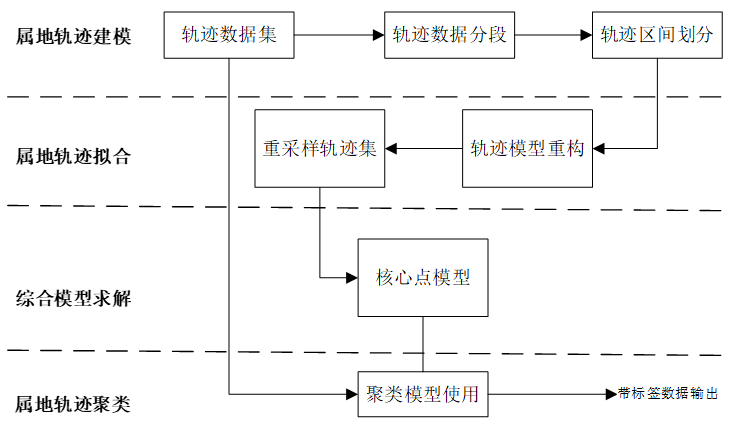
\includegraphics[width=0.8\textwidth]{ch3frame.png}
	\caption{CSD-Clustering 算法框架}
	\label{ch3frame}
\end{figure}

该算法主要包括四个步骤:首先,属地轨迹建模,在各个属地节点对本地的每条轨迹数据进行预处理和抽样(包含轨迹数量抽样和每条轨迹坐标点抽样),并采用多项式函数拟合各抽样轨迹曲线;第二步,轨迹数据重构,每个属地节点将拟合的轨迹函数参数信息发送到中心节点上。第三步,综合模型求解,中心节点根据从接收参数中恢复的轨迹计算聚类结果。最后,模型应用,中心节点将聚类结果返回给每个属地节点,属地节点利用聚类结果应用至不同的业务场景。 

\subsection{属地轨迹地数据预处理}

属地数据预处理可以分为四个步骤,轨迹数量抽样,轨迹点数抽样,分段和分区。如图\ref{ch3pre}所示。
\begin{figure}[H]
	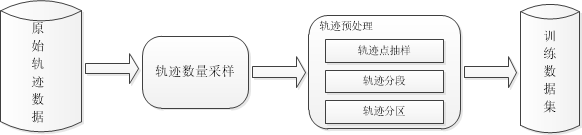
\includegraphics[width=0.8\textwidth]{ch3pre.png}
	\caption{属地轨迹数据预处理}
	\label{ch3pre}
\end{figure}

考虑到更大程度上减少网络中的传输流量和各属地轨迹数据集中存在的数据冗余,属地节点在对轨迹进行建模前进行轨迹数量上的抽样,但应注意,为了保证全局聚类的准确度,分布式平台中的所有属地节点在轨迹数量抽样上的抽样率应保持一致,且抽样得到的轨迹应具有一定的代表性。可以采用一种VQ算法,最典型的VQ算法即是聚类算法。本文采用了k-means聚类算法,其算法流程如算法\ref{kmeans}所示,将属地轨迹数据集输入到k-means算法,得到输出结果,即簇划分$C=\left\{C_1,C_2,...,C_k\right\}$,在每个簇中,采用指定的抽样频率对簇中的轨迹进行随机抽样,对抽样得到的所有轨迹集合中的每条轨迹将执行后续预处理操作。

假设每条轨迹由n个坐标点组成,由于传感器的采样频率一般很高,所以轨迹中相邻点之间的距离相隔很近,针对轨迹拟合问题,适当降低传感器采样频率对于轨迹的大致走势几乎没有影响,为了降低轨迹拟合的计算复杂度,在模型拟合前执行轨迹点数抽样,其抽样频率对于后续轨迹模型的拟合效果将会有很大的影响。

在轨迹建模阶段前,CSD-Clustering需要将每个轨迹分割成连续的轨迹段。其根本原因是,通过函数拟合的曲线必须满足自变量到函数值的唯一映射,当一个自变量对应多个函数值时,函数无法拟合准确。因此,我们采用了轨迹分段的方法,目的是使得轨迹分段曲线任意一个变量中值只对应一个因变量值。

具体地对于每一个时空轨迹矩阵,均有与其对应的速度轨迹V,其刻画了一段时间段内,物体运动的速度变化轮廓。对于上述时空轨迹矩阵P,V定义如下:
\[
\begin{aligned}
	\text{V}&=\left( \text{v}_1,\text{v}_2,...,\text{v}_{n-1} \right)\\
	v_i&=\frac{\left( x_{i+1}-x_i,y_{i+1}-y_i \right)}{\varDelta t}\\
\end{aligned}
\]

其中$v_i$是一个向量,V是一个2×(n-1)矩阵。设有一条由n个轨迹点组成的轨迹P,$T={t_1,t_2,...,t_n}$代表轨迹中坐标点对应的时间,对应速度轨迹$V=(v_1,v_2,...,v_{n-1})$,如果轨迹P划分成两段轨迹,分割时间点为$t_i$,则下列式子需要满足:
\[
\left\{\begin{array}{c}
{v_{1} \cdot v_{k}>0 \quad k=1,2, \ldots, i-1} \\
{v_{1} \cdot v_{i} \leq 0} \\
{v_{i} \cdot v_{n-1}>0}
\end{array}\right.
\]

经过上述分段操作,整个轨迹将被分割成多个子轨迹段。

假设含有n坐标点的子轨迹段通过水平平移到其定义域关于y轴对称时(不考虑两段的开闭区间)所对应的真实函数模型为$f(x)$,并假设$f(x)$n阶可导且可以通过泰勒级数表示,我们试图拟合这个子轨迹段的函数记为$\hat{f}\left( x \right)$ ,毫无疑问,我们希望两者在其定义域内应该尽可能的相似。$f(x)$在x=0处展开的麦克劳伦级数如式\ref{maclaurin}所示,依据其表达式形式可以推出,麦克劳林级数的前n项,即:
\begin{equation}
\label{mac_n}
\hat{f}\left( x \right) =\sum_{i=0}^n{\frac{f^{\left( i \right)}\left( 0 \right)}{i!}}\left( x \right) ^i
\end{equation}

在x=0处的第i阶导数与$f(x)$相等,其中i=0,1,2,...,n,所以式\ref{mac_n}在x=0邻域内与$f(x)$相似度很高,这个邻域范围可以利用幂级数的收敛半径求解方法,若$f(x)$定义域在其收敛半径内,则一定存在一个幂级数能够很好的拟合$f(x)$,反之,如果$f(x)$的定义域超过了其收敛半径所囊括的范围,则式$\ref{maclaurin}$一定无法收敛,故式$\ref{mac_n}$也一定无法收敛,所以任意幂级数前n项拟合$f(x)$时一定存在其第i阶导数与$f(x)$的第i阶导数不相等,因此这个子轨迹段很难通过幂级数前n项式进行拟合。针对这一现象,我们对子轨迹段进行启发式的分区操作,使得通过存在一个幂级数的前n项式能够较好拟合特定区间的轨迹,即限制子轨迹段的定义域长度。

现假设有子轨迹段$\left\{\left(x_{1}, y_{1}\right),\left(x_{2}, y_{2}\right), \dots,\left(x_{N}, y_{N}\right)\right\}$,如果将分段轨迹分成三个轨迹区间:$\left\{\left(x_{1}, y_{1}\right),\left(x_{2}, y_{2}\right), \dots,\left(x_{i}, y_{i}\right)\right\}$,$\left\{\left(x_{i+1}, y_{i+1}\right),\left(x_{i+2}, y_{i+2}\right), \ldots,\left(x_{j}, y_{j}\right)\right\}$和$\left\{\left(x_{j+1}, y_{j+1}\right),\left(x_{j+2}, y_{j+2}\right), \dots,\left(x_{N}, y_{N}\right)\right\}$,则分割坐标i和j应满足:
\[
\begin{aligned}
\left|x_{i+1}-x_{1}\right|&>S\\
\left|x_{j+1}-x_{i+1}\right|&>S      
\end{aligned}
\]

其中S是人工设置的阈值。上述针对分段轨迹的操作成为分区操作,分区操作除了可以缓解上述溢出收敛域可能造成的影响,同时,因为分区轨迹包含的坐标点比分段轨迹少,故可以预设复杂度更低的多项式模型来拟合分区轨迹。

\subsection{属地轨迹拟合}
对第i区间含有k个数据点,$\left\{\left(x_{1}, y_{1}\right),\left(x_{2}, y_{2}\right), \ldots,\left(x_{k}, y_{k}\right)\right\}$,定义损失函数:
\[
\mathrm{L}\left(y_{i}, \hat{f}\left(x_{i}\right)\right)=\left(\mathrm{y_i}-\hat{f}\left(x_{i}\right)\right)^{2}
\]

其中$\hat{f(x)}$表示轨迹拟合函数模型。

将代价函数定义成经验风险函数:
\begin{equation}
\label{ch3costwithoutl1}
\operatorname{cost}(f)=\frac{1}{k} \sum_{j=1}^{k} \mathrm{L}\left(y_{j}, \hat{f}\left(x_{j}\right)\right)
\end{equation}

若$\hat(f)(x)$为n-1次多项式,系数分别为$a_0,a_1,…,a_{n-1}$。

若在此区间使用k-1阶多项式作为轨迹拟合函数模型,即:
\[
\hat{f}\left( \text{x} \right) =a_0+a_1x+\cdots +a_{k-1}x^{k-1}
\]

以此拟合该区间的曲线,将区间的k个坐标带入$\hat{f}(x)$可以得到k个等式,将这k个等式写成矩阵形式即:
\[
\left[\begin{array}{cccc}
{1} & {x_{1}} & {\dots} & {x_{1}^{k-1}} \\
{1} & {x_{2}} & {\dots} & {x_{2}^{k-1}} \\
{\vdots} & {\vdots} & {\ddots} & {\vdots} \\
{1} & {x_{k}} & {\dots} & {x_{k}^{k-1}}
\end{array}\right]\left[\begin{array}{c}
{a_{0}} \\
{a_{1}} \\
{\vdots} \\
{a_{k-1}}
\end{array}\right]=\left[\begin{array}{c}
{y_{1}} \\
{y_{2}} \\
{\vdots} \\
{y_{k}}
\end{array}\right]
\]

记上式中的系数矩阵记为A,易得,$|A^T|$为范德蒙德矩阵,由范德蒙德性质可得:
\[
\left|A^{T}\right|=\prod_{p>q}\left(x_{p}-x_{q}\right)
\]

由于$\mathrm{x}_{0}, \mathrm{x}_{1}, \dots, \mathrm{x}_{k}$彼此不相等,所以行列式$|A^T| \ne 0$,此时存在唯一一个k-1次多项式能够包含所有数据点,此时用k-1阶多项式$\hat{f}(x)$拟合曲线的经验风险为0,拟合的函数曲线穿过每一个坐标点,而且此时求解模型的所有计算量只需计算出系数矩阵A即可。但由于数据不可避免受到噪音污染,我们并不要求拟合的函数曲线严格穿过每一个坐标点,通过求解线性方程组解得的模型往往复杂度很高,可以通过简单实验验证,我们假设在$y=x^2$附近取9个点,通过以上求解线性方程组的方法可以得到一个8阶的多项式,拟合的8阶多项式可以通过所有坐标点,但函数形式却过于复杂,如图\ref{empire0}:
\begin{figure}[H]
	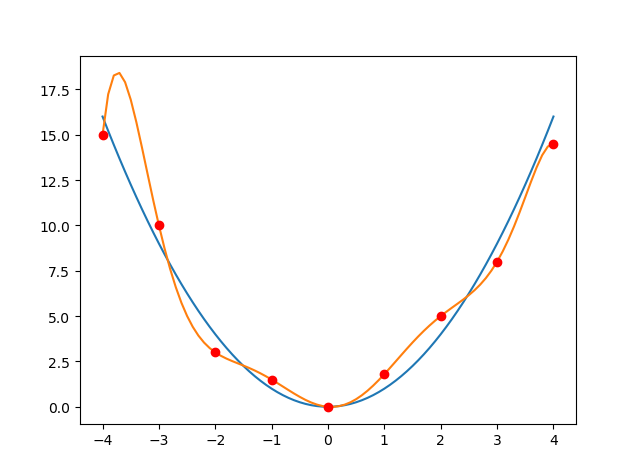
\includegraphics[width=0.8\textwidth]{empire0.png}
	\caption{无正则化拟合}
	\label{empire0}
\end{figure}

而如果我们使用0阶多项式,即常数函数去拟合这条曲线是,此时经验风险非常大,而拟合函数复杂度则很小。为了在满足模型拟合精度的同时避免模型复杂度过高,我们借助最优化理论思想采用经验风险加正则化项的方式,于是代价函数定义为:
\begin{equation}
\label{ch3costL1}
\operatorname{cost}(\hat{f})=\frac{1}{k} \sum_{j=1}^{k} \mathrm{L}\left(y_{j}, \hat{f}\left(x_{j}\right)\right)+\mathrm{C} * J(\hat{f})
\end{equation}

式\ref{ch3costL1}前一项是经验风险,后一项$J(\hat{f})$则是正则化项,也称作结构风险,用来表示轨迹拟合函数$\hat{f}(x)$的复杂度,C为常量,用来调整两者之间关系,若C=0,则代价函数退化成经验损失函数,若C取值很大,则函数模型倾向于选择更简单的模型而不顾拟合准确度。

我们使用参数向量的第二范数来定义$f(\hat{f})$,即:
\[
J(\heat{f})=\sum_{i}^{k}\left|a_{i}\right|_2^2
\]

综上,优化目标定义为:
\begin{equation}
\label{ch3min}
\min \frac{1}{N\left( i \right)}\sum_{j=1}^{N\left( i \right)}{\text{L}}\left( y_i,\text{\hat{f}}_i\left( x_j \right) \right) +\text{C}*J\left( \hat{f}_i \right) 
\end{equation}

其中N(i)表示第i区间数据点的个数,$\hat{f}_i(x)$则表示第i区间多项式拟合函数,其多项式次数为N(i-1)。此类问题属于无约束优化问题,可以采用最速下降来求解局部极小值。

以上方法可以通过另一个角度解释,我们可以将上式看成一般岭回归的形式:
\[
\min _{w}\|X w-y\|_{2}^{2}+\alpha\|w\|_{2}^{2}
\]

我们只是指定了一个明确映射形式的高维映射$\varPhi \left( x \right) =\left( 1,x,x^2,...,x^{k-1} \right) $,故我们求解问题等同于一个指定高维映射的岭回归问题,我们可以通过求解核岭回归的方式求解文中的优化问题。

将通过以上方法可以得到指定区间的函数参数。为了在中心节点能够还原出轨迹数据,除了传递函数参数信息,还需要传输必要的元信息,将元信息和参数信息打包形成的数据结构成为基于复合抽样的轨迹数据单元(CSTD-Unit),其格式如下:
$$
\begin{tabular}{|c|c|c|c|c|}
\hline ID&StartX&EndX&Parament&Alpha\\
\hline
\end{tabular}
$$

数据单元格式字段含义如下:
\begin{itemize}
\item \textbf{ID}:此字段包含了属节点编号、轨迹编号、所处区间
\item \textbf{StartX}:此区间x轴上最小值
\item \textbf{EndX}:此区间x轴上最大值
\item \textbf{Parament}:此区间轨迹拟合函数参数
\item \textbf{Alpha}:节点采用的轨迹点数抽样率
\end{itemize}

各个属地节点把轨迹所有分区坐标信息转化成许多CSTD-Unit传递给中心节点,中心节点通过这种特殊的数据结构能够将轨迹数据进行还原。

\subsection{综合模型求解和模型回传}

在接收到信息后,中心节点根据各个属地节点传输的CSTD-Unit数据单元还原轨迹拟合函数,然后在还原出来的轨迹函数上依照原始数据的采样频率进行等间隔抽样,得到还原出的数据点,以此组成还原数据,从CSTD-Unit数据单元中还原轨迹数据的过程称为轨迹生成过程,轨迹生成过程操作流程如算法\ref{ch3gen}所示。

\begin{algorithm}[H]
	 \KwData{CSTD-Unit数据单元集合U}
	 \KwResult{生成轨迹集合G}
	 \For{unit in U}{
	 		初始化序列ys\;
	 		id = unit['ID']\;
	 		para = unit['Prament']\;
	 		xmin = unit['StartX']\;
	 		xmax = unit['EndX']\;
	 		alpha = unit['Alpha']\;
	 		以1/alpha采样率在区间[xmin,xmax]上进行均匀采样,得到序列xs\;
	 		\For{x in xs}{
	 			lx = np.array([x**i for i in range(len(params))])\;
    			y = np.dot(x,params)\;
    			将y纳入ys\;
	 		}
	 		利用序列xs和序列ys组成轨迹序列L\;
	 	
	 	将轨迹序列L纳入生成轨迹集合G\;
	 }
	 \caption{轨迹生成过程}
	\label{ch3gen}
\end{algorithm}

将恢复的轨迹数据集输入到聚类模型中,本文选择的是K-means++算法,在第二章中描述了k-means算法的具体流程,k-means++只是在k-means基础上针对开始k个均值向量的初始化提供了具体的方法。k-means++方法,尽可能地使初始聚类中心分散开。这种方法首先随机产生一个初始聚类中心点,然后按照概率$P=\omega \sum_i{\left( x-c_i \right) ^2}$选取其他的聚类中心点。其中$\omega$是归一化系数。k-means++初始化操作如下:\\
\begin{algorithm}[H]
	 \KwData{样本集$D=\left\{t_1,t_2,...,t_n\right\}$,簇个数K}
	 \KwResult{簇心向量$\mu=\left\{\mu_1,\mu_2,...,\mu_K\right\}$}
	 从数据集D中随机初始化1个样本,将其作为第一个簇的簇心$\mu={\mu_1}$\;
	 \Repeat{k=2,3,...,K}{
	 	R=D - $\mu$\;
	 	\For{$t_i$ in R}{
	 		计算$P(x_i)$,$P\left( t_i \right) =\omega \sum_{\mu _i\in \mu}{\left( t_i-\mu _i \right) ^2}$,其中$\omega$是归一化系数\;
	 	}
	 	按照R集合中所有点的概率分布选出$\mu_k$,将其加入集合$\mu$\;
	 }
	 \caption{kmeanspp初始化}
\end{algorithm}

全局聚类的具体流程如下:

\begin{algorithm}[H]
	 \KwData{样本集$D=\left\{t_1,t_2,...,t_n\right\}$,簇个数K,阈值S}
	 \KwResult{簇划分$C=\left\{C_1,C_2,...,C_K\right\}$,簇心向量$\mu=\left\{\mu_1,\mu_2,...,\mu_K\right\}$}
	 K=2\;
	 kmeanspp\_initialization(D,K)\;
	 C,$\mu$=kmeans(D,K)\;
	 $DI_K$=$DI(C)$\;
	 flag=true\;
	 \Repeat{flag}{
	 	K=K+1\;
	 	kmeans\_initialization(D,K)\;
	 	C,$\mu$=kmeans(D,K)\;	
	 	$DI_K=DI(C)$\; \\
	 	\If{$DI_K-DI_{K-1}\leqslant S$}{
	 		flag=false\;
	 	}	
	 }
	 \caption{全局聚类流程}
	\label{kmeanspp}
\end{algorithm}

对于k值的选择,在上面的讨论中,我们一直把k当做已经给定的参数。但是在实际操作中,聚类类别数通常都是未知的。如何确定超参数k我们采用如下方法。

我们可以使用不同的k值进行试验,并作出在不同试验中损失函数随k的变化,将损失函数最开始趋向稳定时对应的k值作为我们的最后的取值。如下图\ref{chooseK}所示,分别使用1到7之间的数字作为k值,曲线在k=3处有一个较为明显的弯曲点。故确定k取值为3。
\begin{figure}[H]
	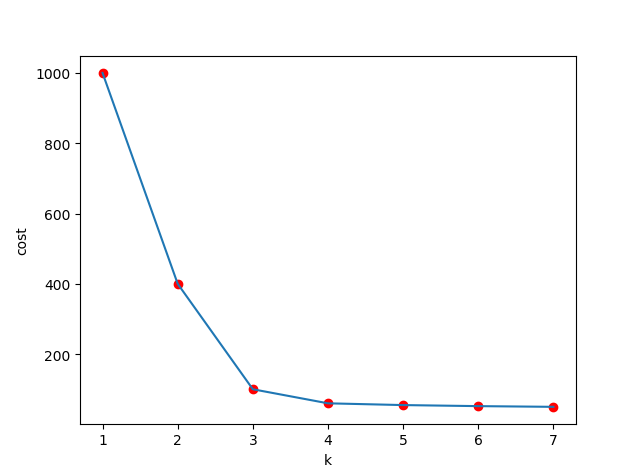
\includegraphics[width=0.8\textwidth]{chooseK.png}
	\caption{k值选择}
	\label{chooseK}
\end{figure}

中心节点计算出k个均值向量后,将k个均值向量回传给各个属地节点,当属地节点侦查到新轨迹时,判断其与回传的k个均值向量的距离来判定是否为异常轨迹:若新轨迹与所有均值向量距离都超过了设定的阈值,则可以判定为轨迹为异常轨迹。


\section{实验与分析}

\subsection{理论分析}

(1)时间复杂度

属地节点时间复杂度分为两个阶段: 轨迹预处理和优化函数求解。

轨迹预处理分为三个步骤,,轨迹数量抽样,轨迹点数抽样,分段和分区。假设轨迹数目为m条,每条轨迹含有坐标点数为n,假设轨迹数量抽样阶段使用k-means算法进行聚类,其复杂度为O(m*n*k*t),k表示簇个数,t是平均迭代次数。轨迹点数抽样复杂度为O(m),
轨迹分段阶段,对于每一条轨迹计算复杂度为O(2*(n-1)),对于m条轨迹则为O(m*2*(n-1)),化简即为O(m*n);区间划分阶段,假设区间中数据点数为i,复杂度为O(2*(i-1)),若对于所有轨迹的所有区间进行分析,则复杂度为O(2*(n-1)*m),化简为O(m*n);优化函数求解阶段,若以最速下降法为例,每次迭代复杂度为O(n*m),若平均迭代次数为t,则在此阶段时间复杂度为O(t*m*n)。综上,函数拟合时间复杂度为O(k*m*n*t)。

中心节点的时间复杂度分为两个阶段:轨迹生成和全局聚类。假设轨迹数目为m,每条轨迹包含n个点,轨迹生成时间复杂度为O(m*n);全局聚类,其时间复杂度为O(m*n*k*t)。

(2)带宽消耗

对于带宽分析,若对于每个节点,若轨迹数量抽样率为$\gamma$,轨迹点数抽样率为$\alpha$;,则对于一个含有m条轨迹、每条轨迹拥有n个数据点、每个数据点维度为2的节点来说,将其传递给中心节点的网络通信量为$(m*n)/(\gamma*\alpha)$;若是传输数据,则网络通信量为m*n*2,故网络通信量的压缩比为$2*\gamma*\alpha$,在此压缩比下,聚类准确度分析将在第五章详细介绍。

(3)隐私性

算法隐私性层面主要从两个角度进行考量:不确定性和覆盖率。

不确定性通过生成轨迹数据与原始属地轨迹数据之间的相似度进行度量,首先,拟合轨迹的多项式模型是通过最小化代价函数得到,而代价函数是由经验损失和正则化构成,所以拟合出的的多项式模型是不经过所有训练数据点的,故原始属地轨迹数据不可能由多项式轨迹准确还原;再者,由于生成轨迹数据是拟合多项式模型在指定区间均匀采样得到,故与原始属地轨迹数据存在一定的差异;但生成轨迹数据与原始轨迹数据在轨迹走向上相似度较高。算法在隐私性的覆盖率方面,由于属地节点在属地轨迹预处理阶段经过了轨迹数量抽样处理,故生成的轨迹数据是无法覆盖所有原始数据的,覆盖率的大小取决于轨迹数量抽样操作的抽样率,抽样率越低则覆盖率越低,反之,覆盖率则越高。

\subsection{实验与分析}
实验是在真实的数据集上进行的,这些数据集包含了在大阪的ATC购物中心的游客的轨迹。在我们的实验中,我们应用了位置x、位置y、人物id字段\footnote[1]{https://irc.atr.jp/crest2010\_HRI/ATC\_dataset/}。经过预处理后,我们选择了2097条轨迹作为原始数据集,每条轨迹包含500个点。

实验系统由三个属地节点和一个中心节点组成。将该算法与集中式聚类方法进行了比较。集中式聚类算法对整个网格化数据集执行标准的k-means算法(baseline), baseline的结果视为最优结果,后续试验中使用的ARI指数则是以 baseline聚类结果作为标签。另一种算法则是本章提出的CSD-Clustering算法。

聚类评估采用两个指标:CR,表示算法的数据压缩能力;ARI,表示聚类结果的精度。

在拟合轨迹曲线前,需要为轨迹区间划分阶段的参数S赋值及拟合轨迹曲线上的结构风险惩罚系数C赋值。

首先对惩罚系数C赋值不同,观察拟合曲线的变化。我们保持轨迹间隔S相同,选择相同的轨迹区间进行观察,将C的值设置为0.001、1、100、10000。结果如图\ref{differentC}所示。
\begin{figure}[H]
	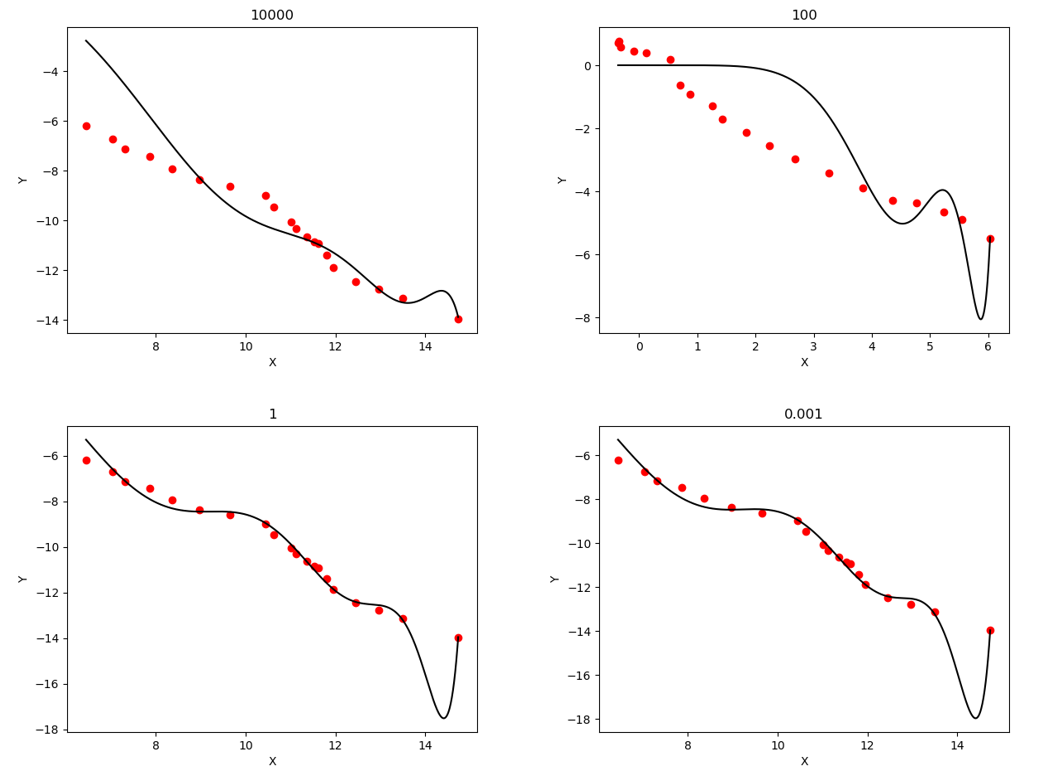
\includegraphics[width=0.8\textwidth]{differentC.png}
	\caption{变量C不同取值的结果}
	\label{differentC}
\end{figure}

从图\ref{differentC}可以看出,随着C值的减小,拟合性能得到改善。然而,当C越来越小时,模型的结构也变得更加复杂。

然后观察参数S对轨迹曲线拟合的影响。我们选择相同的轨迹区间,令S=12和5。结果如图\ref{differentS}所示。
\begin{figure}[H]
	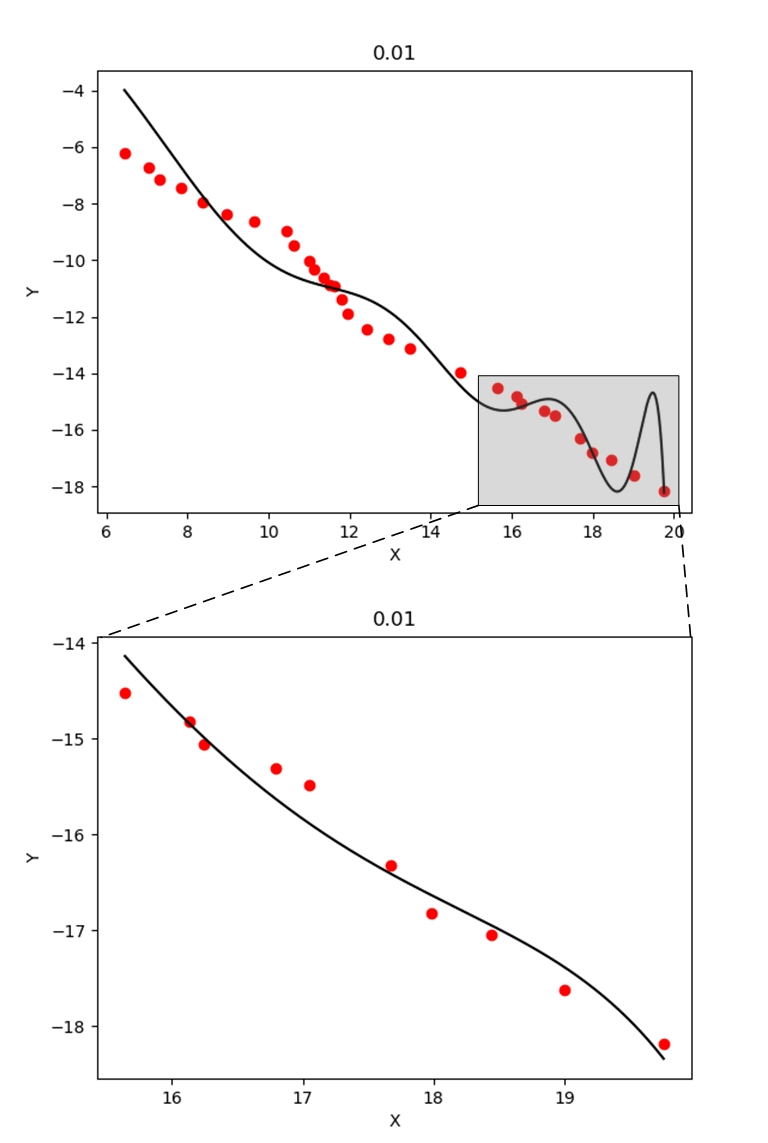
\includegraphics[width=0.5\textwidth]{differentS.png}
	\caption{变量S不同取值的结果}
	\label{differentS}
\end{figure}

从图\ref{differentS}可以看出,上面的那幅图显示当S=12时,拟合曲线的$X\in(6,20)$,下面那幅图显示当S=5时,拟合曲线的$X\in(15,20)$,根据这个结果可以看出,当S越小,曲线拟合得越好。



首先针对原始轨迹数据聚类情况确定全局聚类K值选取,实验中选取不同的K值其损失函数值变化如图\ref{ck}所示,其中损失函数采用均方误差,其表达式如式\ref{kmeanscost}所示。
\begin{figure}[H]
	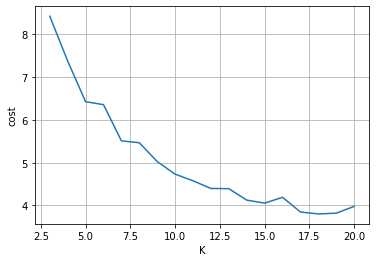
\includegraphics[width=0.8\textwidth]{ck1.png}
	\caption{不同K值损失函数变化}
	\label{ck}
\end{figure}

通过上述实验过程,在后续实验中,设定C取值为1,将K的值设为7。

为了表明轨迹点数抽样率$\alpha$对实验结果的影响,在该实验中,固定轨迹数量抽样率$\gamma=1$,即所有轨迹参与全局聚类,然后将轨迹点数抽样率设置为:1/50、1/20、1/10、1/5和1/2,为了避免在拟合轨迹模型过程中轨迹模型过于复杂,将分段策略设定为固定每段轨迹的点数,本次实验设置分段轨迹点数为5,即轨迹点数抽样率的高低不改变段内轨迹点数,而是改变轨迹分段数。

对于不同轨迹点数抽样率,中心节点生成的轨迹数据与原始轨迹数据对比如图\ref{genTrForDifferentAlpha}所示,其中,图\ref{gen50}表示轨迹点数抽样率为1/50时中心节点生成的轨迹数据,图\ref{gen20}表示轨迹点数抽样率为1/20时中心节点生成的轨迹数据,图\ref{gen5}表示轨迹点数抽样率为1/5时中心节点生成的轨迹数据,图\ref{origin}则表示原始轨迹数据。从图中可以看出,随着轨迹点数抽样率$\alpha$增大,中心轨迹依据参数生成的轨迹数据越接近原始轨迹数据。
\begin{figure}[H]
\subfigure[]{
\label{gen50}
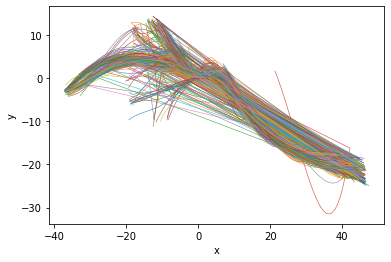
\includegraphics[width=0.4\textwidth]{point_sample_50.png}}
\subfigure[]{
\label{gen20}
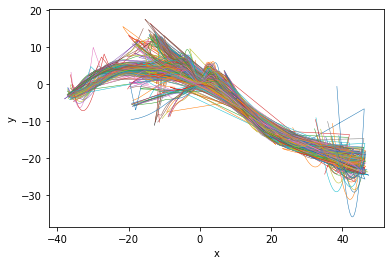
\includegraphics[width=0.4\textwidth]{point_sample_20.png}}
\subfigure[]{
\label{gen5}
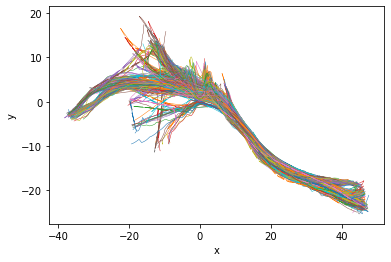
\includegraphics[width=0.4\textwidth]{pic/point_sample_05.png}}
\subfigure[]{
\label{origin}
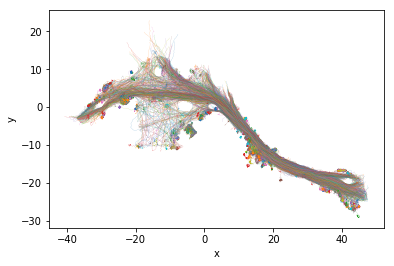
\includegraphics[width=0.4\textwidth]{ch3original.png}}
\caption{不同轨迹点数抽样率下生成轨迹效果对比}
\label{genTrForDifferentAlpha}
\end{figure}

% alpha = [1/50,1/20,1/10,1/5,1/2]
% RI = [0.950 , 0.987 , 0.995 , 0.990 , 0.988]
% ARI = [0.834, 0.958,0.984,0.969,0.963]
% CR = [56.017, 26.452, 14.063 , 7.341, 3.008]

对于不同轨迹点数抽样率,聚类结果如表\ref{differentALPHA}所示,可以看出随着$\alpha$的增加,ARI指数在轨迹采样率为1/50时表现欠佳,当采样率高于1/10后,聚类效果与单中心聚类结果相似程度维持在很高的水平
,而随着轨迹采样率的升高,CR值则随之减小。
\begin{table}[H]
\caption{不同轨迹点数抽样率对比}
\begin{tabular}{|c|c|c|c|c|c|}
\hline
\diagbox{评价指标}{$\alpha$} & 1/50 & 1/20 & 1/10  & 1/5 & 1/2 \\ \hline
ARI   & 0.834 & 0.958 & 0.984 & 0.969 & 0.970\\ \hline
CR   & 56.017  & 26.452 & 14.063 & 7.341 & 3.008\\ \hline
\end{tabular}
\label{differentALPHA}
\end{table}

更高的轨迹点数抽样率意味着更多的轨迹分段,模型对应的参数数量则越多,这将会消耗更多的网络带宽,不同轨迹抽样率对应ARI值和CR值的变化如图\ref{ch3ricr1}所示,ARI用来评价聚类质量,针对网络带宽的压缩率,我们通过自定义的CR指标来衡量。
\begin{figure}[H]
	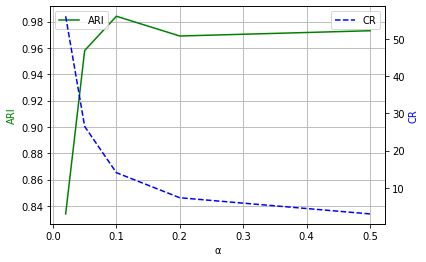
\includegraphics[width=0.8\textwidth]{ch3ex1.png}
	\caption{不同轨迹点数抽样率下ARI和CR变化曲线图}
	\label{ch3ricr1}
\end{figure}


然后实验测试轨迹数量采样率对实验的影响。

此处,设定轨迹点数抽样率$\alpha$=1/5,为轨迹数量抽样率$\gamma$设置不同值:0.1、0.3、0.5、0.7和0.9,验证不同抽样率大小对实验结果的影响。

对于不同轨迹数量抽样率$\gamma$,中心节点生成的轨迹数据与原始轨迹数据对比如图\ref{genTrForDifferentGamma}所示,其中,图\ref{gen01}表示轨迹数量抽样率为0.1时中心节点生成的轨迹数据,图\ref{gen03}表示轨迹数量抽样率为0.3时中心节点生成的轨迹数据,图\ref{gen09}表示轨迹数量抽样率为0.9时中心节点生成的轨迹数据,图\ref{origin}则表示原始轨迹数据。从图中可以看出,随着轨迹点数抽样率$\alpha$增大,中心轨迹依据参数生成的轨迹数据越接近原始轨迹数据。
\begin{figure}[H]
\subfigure[]{
\label{gen01}
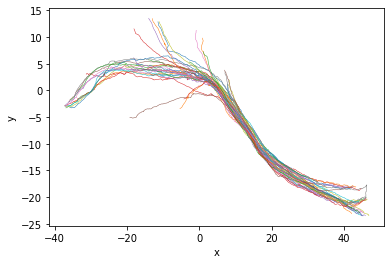
\includegraphics[width=0.4\textwidth]{pic/tr_sample_01.png}}
\subfigure[]{
\label{gen03}
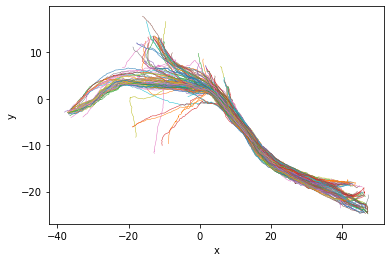
\includegraphics[width=0.4\textwidth]{tr_sample_03.png}}
\subfigure[]{
\label{gen09}
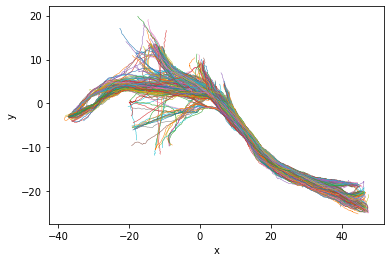
\includegraphics[width=0.4\textwidth]{pic/tr_sample_09.png}}
\subfigure[]{
\label{origin}
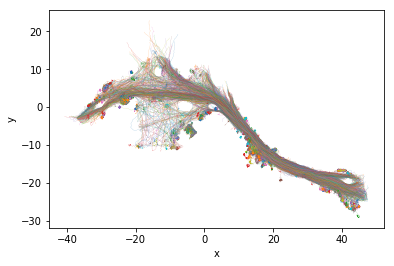
\includegraphics[width=0.4\textwidth]{ch3original.png}}
\caption{不同轨迹数量抽样率下生成轨迹效果对比}
\label{genTrForDifferentGamma}
\end{figure}

% γ = [0.1,0.3,0.5,0.7,0.9]
% ARI = [0.691,0.787,0.838, 0.949, 0.982]
% RI = [0.892 ,0.933 , 0.951 , 0.984 , 0.994]
% CR = [70.168,22.750,13.548,9.689,7.541]

对于不同轨迹数量抽样率,结果数值如表\ref{differentGAMMA}所示,可以看出随着$\gamma$的增加,ARI值越来越大,CR则越来越小。
\begin{table}[H]
\caption{不同轨迹数量抽样率对比}
\begin{tabular}{|c|c|c|c|c|c|}
\hline
\diagbox{评价指标}{$\gamma$} & 0.1 & 0.3 & 0.5  & 0.7 & 0.9 \\ \hline
ARI   & 0.691 & 0.787 & 0.838 & 0.949 & 0.982\\ \hline
CR   & 70.168  & 13.548 & 13.548 & 9.689 & 7.541\\ \hline
\end{tabular}
\label{differentGAMMA}
\end{table}


对于不同轨迹数量抽样率,聚类结果和网络带宽压缩率如图\ref{ch3ricr2}可以看出,随着$\gamma$的增加,聚类的精度也不断增加。同时,随着$\gamma$的增加,也将会带来更大的网络带宽消耗。
\begin{figure}[H]
	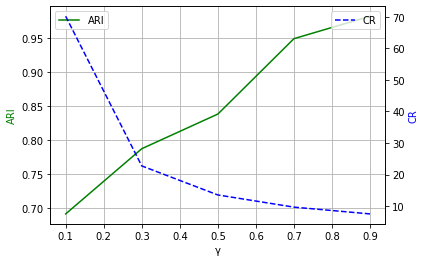
\includegraphics[width=0.8\textwidth]{ch3ex2.png}
	\caption{不同轨迹数量采样率对比}
	\label{ch3ricr2}
\end{figure}

\section{本章小结}

本文提出了一种新型的分布式聚类方案CSD-Clustering,该方案具有节约带宽和保护隐私两方面的优点。网络带宽的降低主要来自三个方面:轨迹集合上的采样,每个轨迹内的部分采样,轨迹模型的拟合函数。此外,该方案还有效地避免了原始数据和直接相关结构信息的传输,加强了隐私保护。评价结果验证了该方法的有效性。